\documentclass[twoside]{report}
\usepackage[utf8]{inputenc}
%\usepackage[english]{babel}
\usepackage{amsthm}
\usepackage{tkz-fct} 
\usepackage{thmtools}
\usepackage[margin=1in]{geometry}
\usepackage{amsmath,amssymb}
\usepackage{multicol}
\usepackage{graphicx}
\usepackage{tikz}
\usepackage{listings}
\usetikzlibrary{positioning} 
\usetikzlibrary{calc,patterns,angles,quotes}
\usetikzlibrary{calc,arrows, arrows.meta}
\tikzset{
  arrow/.pic={\path[tips,every arrow/.try,->,>=#1] (0,0) -- +(.1pt,0);},
  pics/arrow/.default={triangle 90}
}
\usepackage{pgfplots}% also loads graphicx
\pgfplotsset{compat=1.11} %width=10cm,
\usetikzlibrary{backgrounds}
\usepackage{siunitx}
\sisetup{per-mode=fraction} %,fraction-function = \nicefrac}
\DeclareSIUnit{\gallon}{gal}
\usepackage{fancyhdr}
\usepackage{pst-node}
\psset{nodesep=2pt,linearc=2pt,arrows=->,linecolor=blue,arrowinset=0}
\def\lbl#1{\ncput*{\text{\tiny #1}}}
\usepackage{xcolor}
\usepackage{tcolorbox}
\usepackage{lmodern}
\usepackage{relsize}
\newcommand{\highlight}[1]{%
  \colorbox{red!50}{$\displaystyle#1$}}
\usepackage{url}
\usepackage{cancel}
\usepackage{subfig}
\usepackage{mwe}




\usepackage{float}

\usepackage[numbers]{natbib}

\usepackage{setspace}

\usepackage{subcaption}

\usepackage{varwidth}
\usepackage{todonotes}

% set the arrows as stealth fighters (personal preference)
\tikzset{>=stealth}
\captionsetup[figure]{labelfont={bf},name={Figure},labelsep=period}

\declaretheoremstyle[
  spaceabove=6pt, spacebelow=6pt,
  headfont={\color{blue}\fontfamily{cmss}\selectfont\bfseries},
  notefont=\fontfamily{cmss}\selectfont\bfseries, notebraces={(}{)},
bodyfont=\fontfamily{cmss}\selectfont\itshape,
  postheadspace=1em,
]{mystyle}
\declaretheorem[style=mystyle,numbered=no]{definition}
\declaretheorem[style=mystyle,numbered=no]{lemma}

\declaretheoremstyle[
  spaceabove=6pt, spacebelow=6pt,
  headfont={\color{black} \fontfamily{cmss}\selectfont\bfseries},
  notefont=\fontfamily{cmss}\selectfont\bfseries, notebraces={(}{)},
bodyfont=\fontfamily{cmss}\selectfont,
  postheadspace=1em,
  qed=$\triangle$
]{mystyle2}
\declaretheorem[style=mystyle2,numbered=no]{remark}

\declaretheoremstyle[
  spaceabove=6pt, spacebelow=6pt,
  headfont={\color{orange} \fontfamily{cmss}\selectfont\bfseries},
  notefont=\fontfamily{cmss}\selectfont\bfseries, notebraces={(}{)},
bodyfont=\fontfamily{cmss}\selectfont,
  postheadspace=1em,
  qed=$\triangle$
]{mystyle3}
\declaretheorem[style=mystyle3,numbered=no]{example}

\declaretheoremstyle[
  spaceabove=6pt, spacebelow=6pt,
  headfont={\color{blue} \fontfamily{cmss}\selectfont\bfseries},
  notefont=\fontfamily{cmss}\selectfont\bfseries, notebraces={(}{)},
  bodyfont=\fontfamily{cmss}\selectfont\itshape,
  postheadspace=1em,
  qed=
]{mystyle4}
\declaretheorem[style=mystyle4,numbered=no]{law}

\declaretheoremstyle[
  spaceabove=6pt, spacebelow=6pt,
  headfont={\color{blue} \fontfamily{cmss}\selectfont\bfseries},
  notefont=\fontfamily{cmss}\selectfont\bfseries, notebraces={(}{)},
bodyfont=\fontfamily{cmss}\selectfont,
  postheadspace=1em,
  qed=
]{mystyle5}
\declaretheorem[style=mystyle5,numbered=no]{strategy}

\declaretheoremstyle[
  spaceabove=6pt, spacebelow=6pt,
  headfont={\color{blue} \fontfamily{cmss}\selectfont\bfseries},
  notefont=\fontfamily{cmss}\selectfont\bfseries, notebraces={(}{)},
bodyfont=\fontfamily{cmss}\selectfont\itshape,
  postheadspace=1em,
  qed=
]{mystyle6}
\declaretheorem[style=mystyle6,numbered=no]{theorem}


\renewcommand{\qedsymbol}{\rule{0.7em}{0.7em}}
\renewenvironment{proof}{{\bfseries \fontfamily{cmss} \scshape Proof:}}



\newcommand{\reporttitle}{##}
\newcommand{\reportauthor}{Kai Cooper\\Yacine Trad\\Yehao Liu\\ ZachHFT}
\newcommand{\reportsecondauthor}{}
\newcommand{\reportthirdauthor}{}
\newcommand{\reportfourthauthor}{}
\newcommand{\reportfifthauthor}{}
\newcommand{\supervisor}{Dr. Mehdi Gholam \\ Celia Garcia Pareja}

\date{June 2021}

\renewcommand{\chaptername}{Part}
\newcommand{\lap}{\nabla^2}
\newcommand{\dif}[1]{\text{d}#1}

\newcommand{\code}{\texttt}

\definecolor{fcolor}{RGB}{0,255,255}


\begin{document}
\begin{spacing}{1}
% Last modification: 2015-08-17 (Marc Deisenroth)
\begin{titlepage}

\newcommand{\HRule}{\rule{\linewidth}{0.5mm}} % Defines a new command for the horizontal lines, change thickness here


%----------------------------------------------------------------------------------------
%	LOGO SECTION
%----------------------------------------------------------------------------------------

%\includegraphics[width = 4cm]{}\\[0.5cm] 

\center % Center remainder of the page

%----------------------------------------------------------------------------------------
%	HEADING SECTIONS
%----------------------------------------------------------------------------------------

\textsc{\Large École Polytéchnique Fédérale de Lausanne}\\[0.5cm] 
\textsc{\large Department of Mathematics}\\[0.5cm] 

%----------------------------------------------------------------------------------------
%	TITLE SECTION
%----------------------------------------------------------------------------------------

\HRule \\[0.4cm]
{ \huge \bfseries \reporttitle}\\ % Title of your document
\HRule \\[1.5cm]
 
%----------------------------------------------------------------------------------------
%	AUTHOR SECTION
%----------------------------------------------------------------------------------------

\begin{minipage}{0.4\textwidth}
\begin{flushleft} \large
\emph{Authors:}\\
\reportauthor\\ % Your name
\reportsecondauthor\\
\reportthirdauthor\\
\reportfourthauthor\\
\reportfifthauthor
\end{flushleft}
\end{minipage}
~
\begin{minipage}{0.4\textwidth}
\begin{flushright} \large
\emph{Supervisor:} \\
\supervisor % Supervisor's Name
\end{flushright}
\end{minipage}\\[4cm]


%----------------------------------------------------------------------------------------
%	FOOTER & DATE SECTION
%----------------------------------------------------------------------------------------
\vfill % Fill the rest of the page with whitespace

\makeatletter
\@date
\makeatother


\end{titlepage}
\fontfamily{cmss}\selectfont
\tableofcontents




\chapter{Introduction}

\section{Background and scope}
Let's begin by presenting a general overview, during which we'll go through the key-terms needed to understand this project.\\
When faced with a given cryptocurrency, what we see on a price chart is the value of a single \textbf{token}.
The value of a token is equal to the market cap (total value of the network) of a currency divided by the total circulating supply (number of tokens).
Bitcoin has a circulating supply of 19 million tokens but a total supply of 21 million tokens.\\ The difference between the circulating supply and the total supply is the amount still available to be mined, and indicates future inflation. 
$$Token_{BTC}=\frac{MC_{current}}{CS_{current}}$$
\begin{figure}[!htbp]
    \centering
    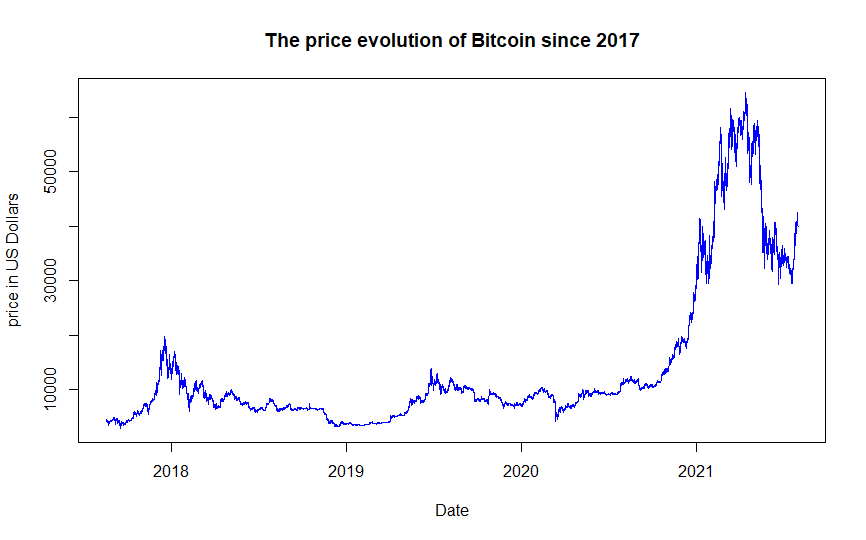
\includegraphics[scale = 0.7]{TestPlots/BTC_overview.png}
    \caption{}
    \label{}
\end{figure}
\\
Just by looking at this chart, one can realise how volatile bitcoin has been and this particularity is shared by many other cryptocurrencies.\\
Bitcoin went from $10K\$$ in September 2020 to over $60K\$$ in April 2021, but also lost half of it's value from April to July 2021.
One can say without doubt that the prices are on a roller coaster, everyone wants to experience the upward trends however the downfalls are extremely scary.\\

Of course, not all cryptos follow the same trends some might be rising while others are crashing, and the goal of crypto-trading is to ride the right wave at the right time, and jump off the ship before it sinks. That is why we will be dealing with crypto pairs which are explained further.\\
The prices fluctuate according to many variables such as news, regulations, announcements, general sentiment etc... Of course risk is involved and that's why the best way to navigate these dangerous waters is to have a set plan and the right logic to follow.







\section{Aim}
\begin{itemize}
    \item 
The goal of this project is to proceed to the analysis of an optimal trading (buy-and-sell) strategy for the market of Cryptocurrencies. We expect such a strategy, if successful, also applicable to the case of traditional stock markets. (note: Cryptocurrencies data are usually more easily and freely available than stock markets data, which are often pricey)
    \item
The first part of the project will consist in showing you how to access the data of all historical data available on Binance. We choose Binance because it is one, if not the only exchange, with a properly working API which also have historical data up to 2017 and for the widest range of cryptocurrency pairs, and therefore the most diverse range of applicable trading strategy (arbitrage, sentiment-driven prices, trends, market making, etc).
    \item{
If you don't want to get your hands dirty (which is understandable) navigating through the code to download the data, simply download a set of the data at this link : \url{https://drive.switch.ch/index.php/s/URDxQbEv8LqSkB2}}

\end{itemize}



\section{The data}
\subsection{Data extraction and processing}
.

\begin{itemize}
\item{To extract the data, you can do so as per the call of \begin{center}\code{getuptodate\_binance\_data.update\_data\_for\_basepair(base\_pair=\'USDT\', nb\_symbols\_limit=5, bin\_size=\'1d\')}\end{center} in \code{get\_ohlc\_historical\_data.ipynb}}.

\item{The data will be saved in a folder named \code{Binance\_OHLC} located within a 'Data' folder within your project folder. If you do not have such folders, create some. (If you are familiar with \code{chdir} python function to change and work with your choice directory you can ignore this remark).}

\item{The code in \code{get\_uptodate\_binance\_data.py} contains a global variable \code{main\_directory} which has the name of my project folder I am working on. I recommend you call your project folders with the same name.}
\end{itemize}




\begin{itemize}
    \item 
We use the \code{clean\_csv} function to clean the newly downloaded data file. In particular, we setup timestamp in datetime format, to allow us to have an easier handling of the data later on.
    \item
We also select a subset of the columns of interest to us. In particular we keep keep the following columns: ['timestamp', 'open', 'high', 'low', 'close', 'volume', 'time\_diff\_in\_days', 'time\_diff\_in\_min'].
    \item
Note that we have never encountered any NA values or other seemingly out-of-place values that would need to be rejected. Indeed, so called 'out-of-place values' or any other outliers kind of value are strong indicators which require further investigations and may be relevant to dedicated algorithmic trading strategies. We absolutely do not want to remove them as we may be tempted to do in some other contexts in data science.
    \item
Discrepancies in the timestamp of our data : Missing time periods. Every once in a while there is a major crash in cryptocurrencies market (i.e. prices dropping significantly). This leads to a massive amount of people trying to connect to the cryptocurrencies exchange platforms to try to sell (or buy) some cryptocurrencies.This often results in the exchange becoming unavailable, their server not being able to handle so many connections attempts at once. This explains the missing data in historical cryptocurrencies prices data (It can be for a couple of minutes up to a couple of hours). We therefore compute 'time\_diff\_in\_days' and 'time\_diff\_in\_min' to spot any such discrepancies in the timestamp.
    \item
You can find the code in the \code{get\_uptodate\_binance\_data.py} file

\end{itemize}


Going further...

\begin{itemize}
    \item 
Once an analysis is performed on a dedicated dataset (e.g. 1 hour BTC/USDT historical data), the same statistical analysis can be performed over any dataset (e.g. 1 minute ETH/CHF historical data), since the data structure (i.e. the columns, open, high, low, close) is the same. We will do so later on in the project.
    \item
We downloaded the data for hundreds of cryptocurrency pairs over various timeframe (1 day, 1 hour, 1 minute, etc) so that we can perform meta-analysis and/or repeat the small single-pair dataset analysis over all other sets

\end{itemize}



\subsection{Data transformation}

The goal of this project is to proceed to the analysis of an optimal trading (buy-and-sell) strategy for the market of Cryptocurrencies. Our analysis will be made on cryptocurrency pairs.\\
These pairs allow us to compare costs between different cryptocurrencies. They are helpful for illustrating the relative worth of coins. For example,the question how much Bitcoin (BTC) equals in Ethereum (ETH) will be answered by the value of the pair BTC/ETH.
In this report we are dealing with the BTC/USDT pair. USDT stands for Tether which is a stable coin in which each token is backed by a U.S Dollar.\\
The price of a token depends on the market cap of the currency and how many tokens are issued. And since there are hundreds of cryptocurrencies dealing with their prices can become very cumbersome and lack clarity. For that very reason, we have chosen to deal in our analysis with log-returns.
Indeed, the price of a currency is not what is of interest to us but rather it's evolution. By studying prices we would be confronted with values that don't have an intrinsic meaning, However with log returns we will have an idea of the evolution in percentages, which is way more useful. To sum it up, this allows measuring a lot of variables in a comparable metric, thus enabling evaluation of analytic relationships amongst two or more variables despite originating from price series of unequal values. \\
Concretely, if we are doing our study on a currency at time $i$ which is valued at price $p_i$. The log-return for the period $t$ is:
$$\log\left(\frac{p_i}{p_{i-t}}\right)$$\\

Another important property is the additivity of the log-return. If our price at $t_1$ is $p_1$, it changes to $p_2$ at $t_2$ and move to $p_3$ at $t_3$. The log return from $t_1 $ to $t_2$ is $\log (p_2) - \log (p_1)$, the log return from $t_2 $ to $t_3$ is $\log (p_3) - \log (p_2)$. Therefore, it is clear that the log return from $t_1 $ to $t_3$ is $\log (p_3) - \log (p_1)$. This can be calculated easily. However, if we use simple return, the return should be $p_3/p_1$ instead of $p_3/p_2 + p_2/p_1$. Hence, log-return is easier to apply to real data.

 An interesting observation one can make when plotting the log-returns is that they are supposed to be normally distributed, however when looking at Figure 1.1 we can see that the mean is slightly tilted to the positive side which indicates that BTC has been a good investment overall.
 
 
 \section{Exploratory data analysis}
.
\subsection{Distribution of prices and returns}

\begin{figure}[!htbp]
    \centering
    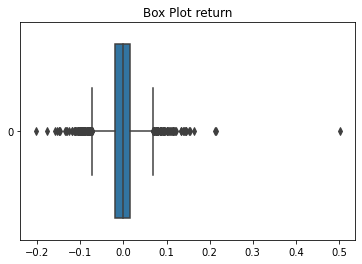
\includegraphics[scale = 0.5]{Images/Box Plot of Return.png}
    \caption{Box plot of log-return}
    \label{log return box}
\end{figure}

Figure \ref{log return box} shows the box plot of log-return of BTC. As can be seen from the graph, there are many outliers of the box plot. So it is reasonable to say that the distribution of log-return is not a normal distribution. More evidence will be given in the following sections.

\begin{figure}[!htbp]
    \centering
    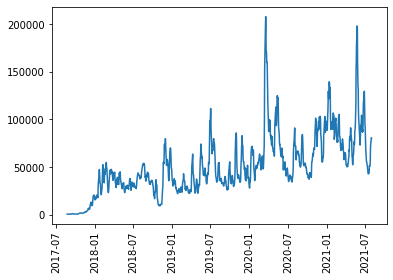
\includegraphics[scale = 0.5]{Images/Volume Rolling Average.png}
    \caption{7 day rolling average of the volume}
    \label{7day rolling volume}
\end{figure}

Figure \ref{7day rolling volume} is about 7 days rolling average of the volume. From this figure, we see that the volume oscillate during our examining period. The volume sometime change drastically for a certain day. However, with the existence of up and down signals, we see there is a trend of volume increasing from the beginning of 2017-07 to 2021-07.


\subsection{Mean and Median hourly BTC/USDT log-return by day, by week, and by month}

In the following we show historical hourly log-return based on the trading day, the trading week, or the trading month.
\\ \\
We can notice that historically, Thursday is a bad trading day, and if historical trends are any indication of future trends, we may want to consider avoiding trading on this particular day.
\\ \\
Similarly, we see that the months of March and September are historically quite bad months to trade and we may want (assuming this trend will repeat in the future) selling our BTC assets in the beginning of these months and buying back at the end of these months.
\\ \\
We display the charts below.
\begin{figure}[!htbp]
    \centering
    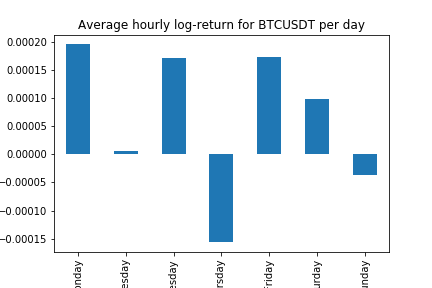
\includegraphics[scale = 0.5]{Images/Average hourly log-return for BTCUSDT per day.png}
    \caption{Average hourly log-return for BTCUSDT per day}
    \label{Average hourly log-return for BTCUSDT per day}
\end{figure}

\begin{figure}[!htbp]
    \centering
    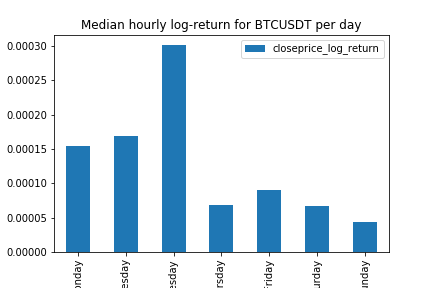
\includegraphics[scale = 0.5]{Images/Median hourly log-return for BTCUSDT per day.png}
    \caption{Median hourly log-return for BTCUSDT per day}
    \label{Median hourly log-return for BTCUSDT per day}
\end{figure}

\begin{figure}[!htbp]
    \centering
    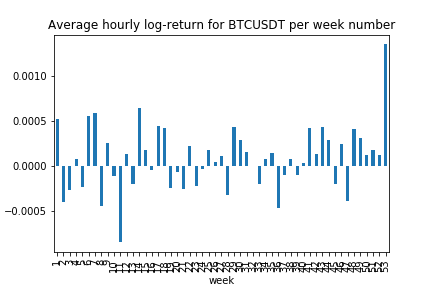
\includegraphics[scale = 0.5]{Images/Average hourly log-return for BTCUSDT per week number.png}
    \caption{Average hourly log-return for BTCUSDT per week number}
    \label{Average hourly log-return for BTCUSDT per week number}
\end{figure}

\begin{figure}[!htbp]
    \centering
    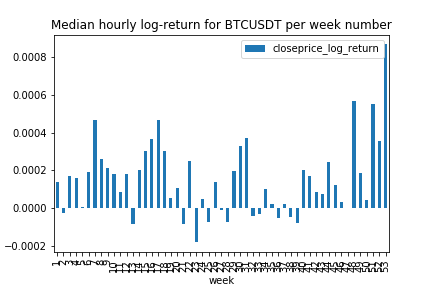
\includegraphics[scale = 0.5]{Images/Median hourly log-return for BTCUSDT per week number.png}
    \caption{Median hourly log-return for BTCUSDT per week number}
    \label{Median hourly log-return for BTCUSDT per week number}
\end{figure}

\begin{figure}[!htbp]
    \centering
    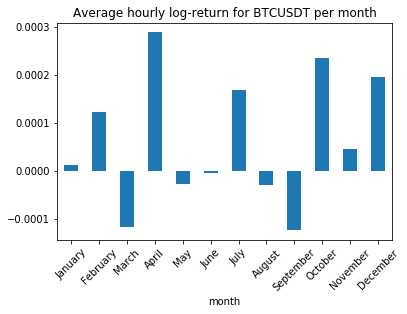
\includegraphics[scale = 0.5]{Images/Average hourly log-return for BTCUSDT per month.png}
    \caption{Average hourly log-return for BTCUSDT per month}
    \label{Average hourly log-return for BTCUSDT per month}
\end{figure}

\begin{figure}[!htbp]
    \centering
    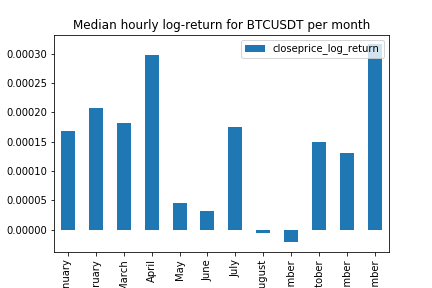
\includegraphics[scale = 0.5]{Images/Median hourly log-return for BTCUSDT per month.png}
    \caption{Median hourly log-return for BTCUSDT per month}
    \label{Median hourly log-return for BTCUSDT per month}
\end{figure}


\subsection{Analysis of extremes}

In finance, the question of extreme values is indubitably an important one. For example: stock market crashes, interest rates ad  insurance pricing based on life expectancy are all fields in which it would be necessary to consider rare events. The analysis of cryptocurrency trajectories is no different, indeed, sudden but large deviations in the trajectory of cryptocurrency prices would certainly be of interest to a trader. 

In light of this, it is not unnatural to ask the corresponding statistical question in the context of extremes. In Figure \ref{fig:hist_logreturn_17_21}, we can see that the distribution of log returns for our data set admits very heavy tails. In this dataset there are many statistically anomalous results which skew the data, but even upon their removal, the data remain strongly skewed, see Figure \ref{fig:distplots_sans_outliers}, the data still exhibit this skewed behaviour. This sparks interest in using extreme value theory to aid our understanding of this behaviour.\\

If we observe a trajectory of prices $p_t$, for $t$ an index of time (e.g. prices per minute or hour, etc.), by assuming they come from a random sample, we can aim to fit their scaled extreme, either maximum or minimum, to a distribution of the following type \[
G(x; \eta, \tau, \xi) = \begin{cases}
\exp\left[-\left\{1+\xi(x-\eta)/\tau\right\}_+\right], & \xi \ne 0\\
\exp\left[-\exp\left\{-(x-\eta)/\tau\right\}\right], & \xi = 0,
\end{cases}
\]
where $\eta, \tau$ and $\xi$ are location, shape and scale parameters respectively. Studying maxima in this way is called the \textbf{block maxima approach}, since one groups data and considers fitting the distribution to the maxima across all groups, for example: maximum price over one day, where the prices are indexed by hours.

The goal now, therefore, is to fit this model to our data, i.e. by finding the unknown parameters. To this end, we use the $\code{R}$ package $\code{evd}$ which gives useful functions for extremal modelling and makes plotting diagnostics straightforward. 
\begin{figure}
    \centering
    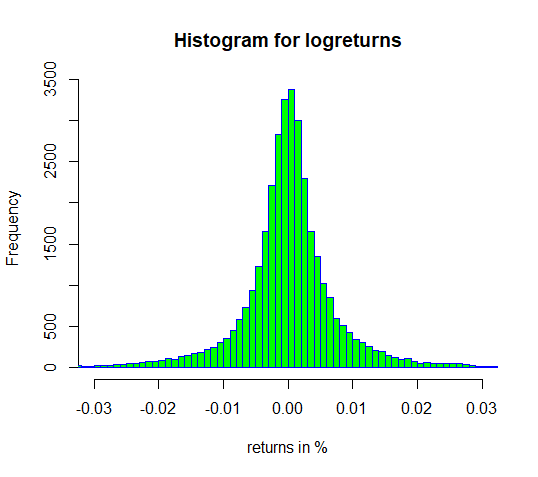
\includegraphics[width=\linewidth, height=3.5in]{TestPlots/Histogram log-returns2.png}
    \caption{Distribution of log returns using data from August 2017 to August 2021. The distribution shows some quite heavy tails.}
    \label{fig:hist_logreturn_17_21}
\end{figure}

\begin{figure}
    \centering
    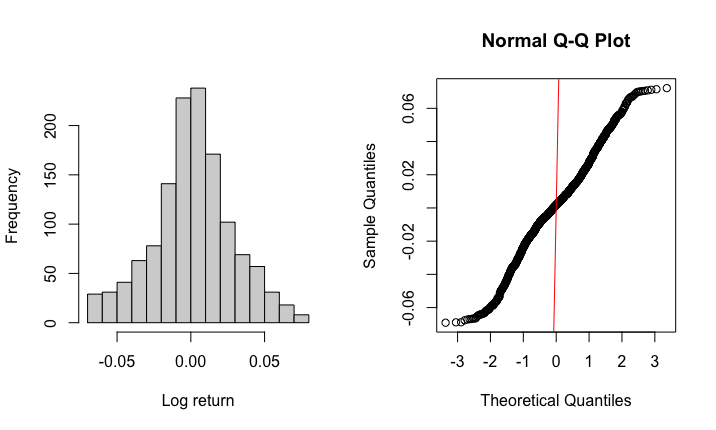
\includegraphics[width=\linewidth]{Extremal Modelling/distplots_sans_outliers.png}
    \caption{Distribution of log returns having eliminated outliers and a QQ plot of the data against a standard normal random variable. Clearly the data is still heavily tailed.}
    \label{fig:distplots_sans_outliers}
\end{figure}



.

\chapter{Social media's influence on cryptocurrency prices}
.
\section{Price versus human behaviour}

\section{Twitter}
Twitter is an American microblogging and social networking service on which users post and interact with messages known as "tweets". Users can post, like, and share (or retweet) tweets.
From common people to highly influential billionaires, everyone has something to say and millions of people react and share their opinions on that platform. Donald Trump for instance has used it to communicate with the American citizens during his mandate. And we can say that the influence happening on twitter is unquestionable.\\

Users interact with Twitter through browser or mobile frontend software, however in order to collect data from that platform programmatically one has to do it via its APIs.
We have used the python library snscrape.modules.twitter to collect the data we needed.\\


\section{Medium}
\section{Reddit}
...
Reddit is the Internet's forum. It serves as a hub for discussion on just about anything you can think of. Naturally, therefore, cryptocurrency enthusiasts will discuss trends, advice and more in the many dedicated fora such as 'r/Cryptocurrecy' or 'r/Bitcoin'. For this reason, it is not hard to imagine that there are more prominent members of the community who feature across several fora and make frequent contributions to the community. Over time, these people may gain a reputation for some type of expertise. Such people, like in the Twitter section, we will call \textbf{influential}, or in the noun form: \textbf{influencers}. 

But how can we identify such people? Reddit is largely anonymous, and many important members of the community aren't as easily identifiable as Elon Musk. Therefore, tt is important to not treat this question subjectively, since that could lead to the omission of potentially important authors whose contributions to the network of crypto traders have been valued. Consequently, we make a superficial\footnote{due to time constraints} use of network science to locate these users. 
\subsection{Reddit as a social network}\label{sec:redditSN}
Reddit, by definition, is a type of social network. Therefore it lends itself to being represented mathematically in this way. However, there is a large variety at disposal here. To list some examples, one could form: a network of fora which share users; a network of users and those who comment on their posts or a network of fora and their users. Each of these cases present distinct sets of network elements: the first, a set of subreddits; the second, a set of users while the third is a mélange of the two. 

To illustrate the sheer versatility of this approach, we begin by forming several networks based on subreddits and users centered at the \textbf{r/CryptoCurrency} subreddit. The data were accessed using the extensive \code{praw} library in Python, which is used for webscraping essentially all publicly visible Reddit data. 

Firstly, we access a set of users who have posted in the r/CryptoCurrency subreddit across the top $500$ submissions in recent history. Their activity in the subreddit is shown in Figure ... 

\begin{figure}
    \centering
    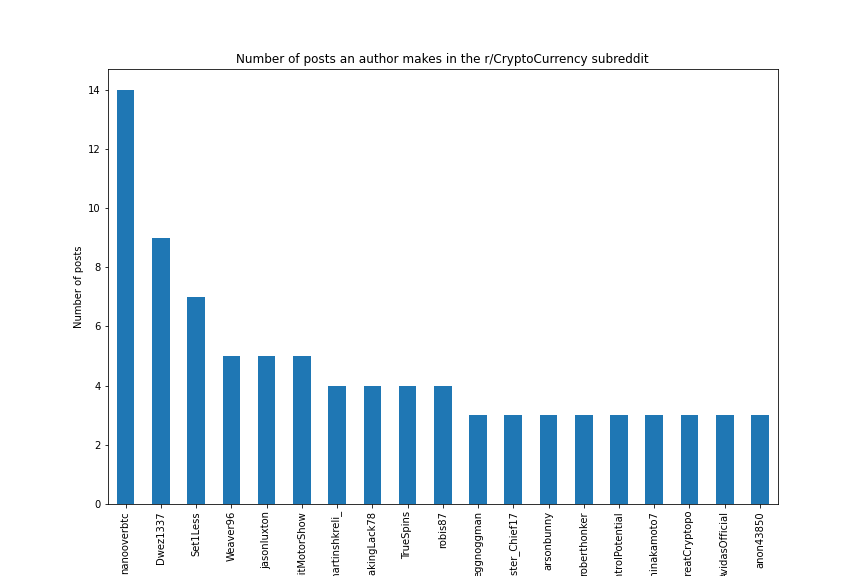
\includegraphics[width=\linewidth]{Reddit_Analysis/Network_Analysis/num_posts_r_crypto.png}
    \caption{Caption}
    \label{fig:num_posts_r_crypto}
\end{figure}

\begin{figure}
    \centering
    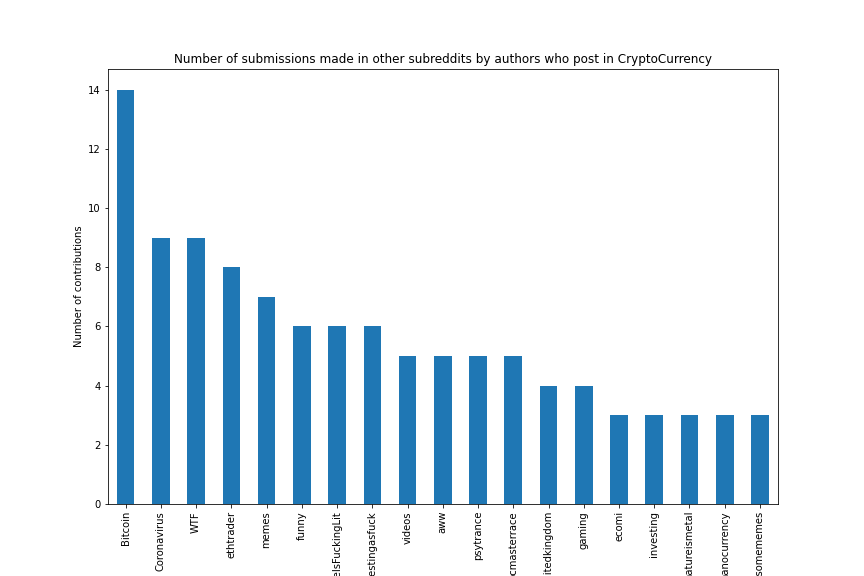
\includegraphics[width=\linewidth]{Reddit_Analysis/Network_Analysis/other_subs_contributions.png}
    \caption{Caption}
    \label{fig:other_subs_contributions}
\end{figure}

\begin{figure}
    \centering
    \includegraphics{}
    \caption{Caption}
    \label{fig:my_label}
\end{figure}

\begin{figure}

\begin{minipage}{.5\linewidth}
\centering
\subfloat[]{\label{main:a}\hspace{-2em} \includegraphics[scale=.25]{Reddit_Analysis/Network_Analysis/author_projection.png}}
\end{minipage}%
\begin{minipage}{.5\linewidth}
\centering
\subfloat[]{\label{main:b}\includegraphics[scale=.25]{Reddit_Analysis/Network_Analysis/subreddit_projection.png}}
\end{minipage}\par\medskip
\centering
\subfloat[]{\label{main:c}\hspace{-2em}\includegraphics[scale=.4]{Reddit_Analysis/Network_Analysis/bipartite_demonstration.png}}
\caption{my fig}
\label{fig:main}
\end{figure}

Of course, the goal is to find out who are the most important users in the cryptocurrency reddit network. Therefore, we then access the subreddits in which these authors are most active --- unsurprisingly, we find other cryptocurrency dedicated subreddits such as r/Bitcoin and r/ethereum. To analyse this structure more deeply, we create a social network, $G$, connecting these authors and subreddits. The first network we construct is formed in the following way: if redditor $r$ posts in subreddit $s$, then we connect $r$ and $s$ by a \textbf{link}, which we may denote $r \sim s$ (read as: $r$ is linked to $s$). We say that the \textbf{nodes} of this network are the elements connected via a link. One should notice that a network constructed in this way has a special property. It is possible to separate the set of nodes $V$ of $G$ into two groups $R$ and $S$ where there exist no links between pairs of nodes where each node belongs to the same set: such network are called \textbf{bipartite}.

The substructures of networks of this type are often of interest to analysts. Indeed, such networks admit two \textit{projections} which encapsulate the substructure. For example, we can form a network between subreddits $s, s' \in S$ where $s \sim s'$ whenever there is an $r$ such that $r \sim s$ and $r\sim s'$. In words: if a redditor has posted in both subreddits $s$ and $s'$, then we can create an edge between them, producing the graph in Figure ... 

What can we learn from such a network? For instance, it is of no doubt an interesting question to ask whether the subreddit projection of the bipartite network form groups of subreddits within themselves. There are many algorithms out there to detect \textbf{communities} within a network, and some are identified here. In this particular case we would hope to find that financially inclined subreddits  would form communities. 

To make an objective conclusion on where communities form, it is necessary to attribute a degree of importance or \textbf{centrality} to nodes and edges within a network, some measures of centrality are detailed in Table \ref{table:centralityMeasures}

\begin{table}[htbp]
\centering
\begin{tabular}{|l|p{0.65\linewidth}|}
\hline
\multicolumn{1}{|c|}{\textbf{Centrality Measure}} & \multicolumn{1}{c|}{\textbf{Qualitative Description}}
\tabularnewline \hline
      Degree centrality & the fraction of nodes it is connected to. It is used to determine what nodes are most connected. \\
      \hline
      Betweenness  centrality & measures the number of shortest paths that the node lies on. This centrality is usually used to determine the flow of information through the graph. The idea here is that even while the node may not have the largest degree, it is important to the network if it lies on many of the shortest paths connecting two nodes in the graph. Think of transoceanic internet traffic and the router network: routers connecting the US and the UK will be very important to this network and indeed will separate two communities, even if in those communities their degree is not as high as elsewhere. It is these nodes one wishes to identify.\\
      \hline 
      Eigenvector centrality & Measures the node’s relative influence in the network, or how well a node is connected to other highly connected nodes. \\
      \hline 
      Edge betweenness centrality & ranks edges by the number of shortest paths passing through the edge, similar to betweenness centrality but for edges.
 \tabularnewline \hline
\end{tabular}
\caption{}
\label{table:centralityMeasures}   
\end{table}




...
\begin{table}[htbp]
\centering
\begin{tabular}{|l|p{0.65\linewidth}|}
\hline
\multicolumn{1}{|c|}{\textbf{Subreddit}} & \multicolumn{1}{c|}{\textbf{Centrality Measure}}
\tabularnewline \hline
 \tabularnewline \hline
\end{tabular}
\caption{Various centrality scores for the subreddit projection $G_S$ of our original network $G$.}
\label{table:centralitySubreddits}   
\end{table}

\subsection{Assessment of profit and loss against influential redditors}\label{sec:redditPNL}
We now use the ideas presented in section \ref{sec:redditSN} to identify the most influential reddit authors present in $n$ popular subreddits. We begin by forming an author--commenter network, where we form a \textbf{directed} graph such that if redditor $r$ comments on a post of redditor $r'$ then $r \rightarrow r'$. Indeed, we encode now each link with a direction, hence the term \textbf{directed} network. We achieved this via the \code{praw} library by extracting the top ... posts in the cryptocurrency related subreddits combined with their author and commenter data. 

To study and visualise the graph, we explored the R packages \code{igraph}, \code{ggraph}, \code{visNetwork}, \code{graphlayouts} [...] extensively. Moreover, a very recent development in the field of network science has constructed the centrality measure, \textbf{Integrated Value of Influence} \cite{IVIpatterns}, which uses various statistical measures to compare various centrality measures for a graph to determine the most influential nodes, see Figure ... Fortunately, the authors of that paper have created a comprehensive R package called \code{influential} whose function \code{ivi} does the heavy lifting for us. 



Please do visit the site \url{https://kcvis.shinyapps.io/network_analysis/} to play around interactively with the network created. 







\end{spacing}
\end{document}
